%%%%%%%%%%%%%%%%%%%%%%%%%%%%%%%%%%%%%%%%%%%%%%%%%%%%%%%%%%%%%%%%%%
%%%%%%%% ICML 2015 EXAMPLE LATEX SUBMISSION FILE %%%%%%%%%%%%%%%%%
%%%%%%%%%%%%%%%%%%%%%%%%%%%%%%%%%%%%%%%%%%%%%%%%%%%%%%%%%%%%%%%%%%

% Use the following line _only_ if you're still using LaTeX 2.09.
%\documentstyle[icml2015,epsf,natbib]{article}
% If you rely on Latex2e packages, like most moden people use this:
\documentclass{article}

% use Times
\usepackage{times}
% For figures
\usepackage{graphicx} % more modern
%\usepackage{epsfig} % less modern
\usepackage{subfigure} 

% For citations
\usepackage{natbib}

% For algorithms
\usepackage{algorithm}
\usepackage{algorithmic}

% As of 2011, we use the hyperref package to produce hyperlinks in the
% resulting PDF.  If this breaks your system, please commend out the
% following usepackage line and replace \usepackage{icml2015} with
% \usepackage[nohyperref]{icml2015} above.
\usepackage{hyperref}

% Packages hyperref and algorithmic misbehave sometimes.  We can fix
% this with the following command.
\newcommand{\theHalgorithm}{\arabic{algorithm}}

% Employ the following version of the ``usepackage'' statement for
% submitting the draft version of the paper for review.  This will set
% the note in the first column to ``Under review.  Do not distribute.''
\usepackage{icml2015} 

% Employ this version of the ``usepackage'' statement after the paper has
% been accepted, when creating the final version.  This will set the
% note in the first column to ``Proceedings of the...''
%\usepackage[accepted]{icml2015}



% The \icmltitle you define below is probably too long as a header.
% Therefore, a short form for the running title is supplied here:
\icmltitlerunning{Final Project: STAT 241a}

\begin{document} 

\twocolumn[
\icmltitle{Final Project: STAT 241a \\ Using Hidden Markov Model \\ 
to Estimate Functional Networks in fMRI Data}

% It is OKAY to include author information, even for blind
% submissions: the style file will automatically remove it for you
% unless you've provided the [accepted] option to the icml2015
% package.
\author{Chris Gagne}{Chris Gagne, UC Berkeley Psychology Department }



% You may provide any keywords that you 
% find helpful for describing your paper; these are used to populate 
% the "keywords" metadata in the PDF but will not be shown in the document


\vskip 0.3in
]


\section{Project Overview}

For my project, I (1) implemented a model borrowed from (Liu 2011; Liu 2014), (2) tested my implementation using simulations, and (3) applied it to my fMRI dataset. Throughout the process, I explored in depth several concepts we touched upon in the course.


\section{Background}

An important organizing principle of the human brain is that sets of regions tend to co-activate during a wide range of tasks. For example, regions in medial frontal cortex tend to correlate with subcortical structures, while lateral frontal regions tend to correlate with motor cortex. The first set of regions is though to be responsible for emotional processing, while the later is thought to underly goal-directed motor behavior. Using fMRI, we can identify these 'functional networks' in human brains and study how they change as people perform different tasks. 

To locate networks, voxels (3-D pixels) are clustered (i.e. assigned network labels) based on similarities in their time-series. In my dataset, for example there are 60,000 voxels per 'image' and an image collected every 2s for a 30 minutes. 

Common methods for clustering voxels based on similar time series are ICA and K-means. Although these methods perform well, they do not take advantage of the spatial information about the voxels and the fact that functional networks tend to consist of voxels that are spatially contiguous. Therefore, Liu 2011 (among others) proposed to use a Markov Random Field to incorporate spatial information into a clustering model. I chose to implement this model because of its relevance to the course. 


\section{Model} 

\begin{figure}[ht]
\vskip 0.2in
\begin{center}
\centerline{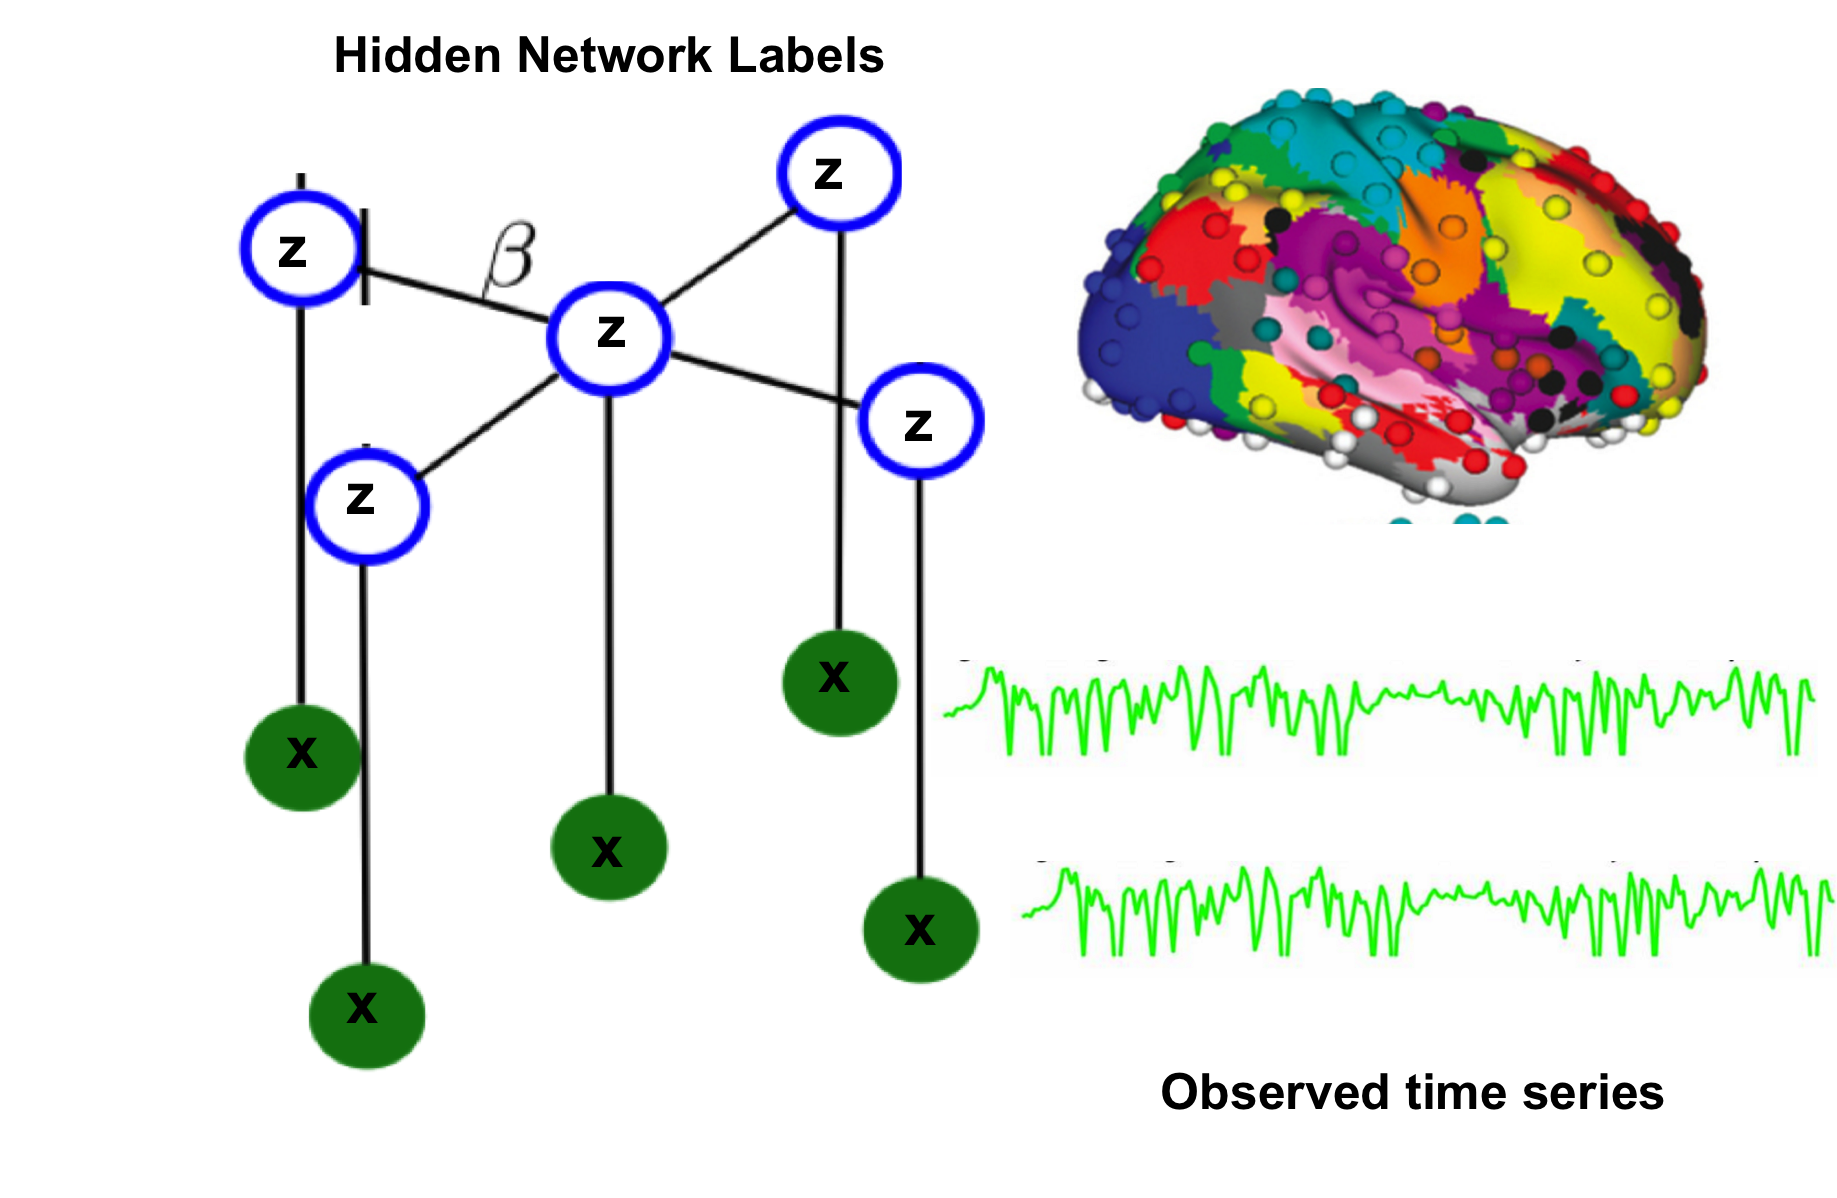
\includegraphics[width=\columnwidth]{Model}}
\caption{(left) Graphical Model; $x_i$ are conditionally independent from one another given the network labels $z_i$ and these are conditionally independent of other $z_{-i} $ given their neighbors $N$. (right) an example of functional networks estimating using a different method (Yeo 2011). }
\label{Model}
\end{center}
\vskip -0.2in
\end{figure} 

In the model of Liu 2011, voxels are clustered using a generalization of the hidden markov model (which itself is a generalization of the mixture model), in which the Markovian assumption is made about spatially adjacent voxels rather than temporally sequential observations. Specifically, the hidden variables are network labels for each voxel ($ Z = {z_1,z_2,z_3... }$), and the observed variables are the time courses for those voxels ($ X = {x_1,x_2,x_3...} $). The network label variable for a voxel is conditionally independent of other voxel labels given its that voxel's neighbors. In this way, the model incorporates the assumption that a voxels network should be similar to its spatial neighbors. See Figure~\ref{Model}

As a mixture model, the total probabilistic model for the observed data X is a sum over the joint of the observed variables and hidden variables: 

$$ p(X) = \sum_Z p(X,Z) $$
$$ p(X,Z) = p(Z) \prod p(x_i | z_i)  $$

The modeling \textbf{goal} will be to infer the most likely values for the hidden network labels (Z) after estimating the model parameters.  
 

\subsection{Prior for hidden variables} 

The probability of the hidden variables is represented as an undirected  graphical model (referred to as Markov Random Field in Liu 2011). The particular form of the cliques potentials chosen leads to what is known as a Potts model. I will show this below: 

We can write the joint distribution for an undirected model as a product of clique potentials. 
$$ P(Z) = \frac{1}{C} \prod \Psi(z)  $$
If the potentials are chosen to be exponentials, we get, 
 $$ = \frac{1}{C} \prod e^{h(x)} $$
$$  = \frac{1}{C}  e^{\sum_i h(x)}  $$
which is know as the Boltzmann or Gibbs distribution. The function in the exponential is known as the energy function. For this model, Liu 2011 choose the following energy function creating what is known as the Potts model (i.e. which is a multi-class Ising Model): 
$$ P(Z)  = \frac{1}{C} e^{ - \beta \sum_i \sum_{j  \in N_j} \delta(z_i \neq z_j)} $$

The probability of states is determined by the number of neighboring nodes $ N $ that share the same state (kronecker $\delta $)

More informatively, by Gibbs-Markov equivalence, we can write the conditional distribution of each $z_i$ as:

\begin{equation}
P(z_i|z_{-i} )  = \frac{e^{ - \beta \sum_{j  \in N_j} \delta(z_i \neq z_j)}}{\sum_l e^{ - \beta \sum_{j  \in N_j} \delta(l \neq z_j)}}  
\end{equation} 

which will be useful for model estimation. 


\subsection{Likelihood for observed time-series} 

Liu 2011 use a von-Mises Fisher distribution for the emission distribution $ p(X|Z)$. fMRI time-series vectors are usually demeaned and normalized to have unit length. Therefore, the data lies on a t-1 dimensional hypersphere. Von-Mises Fisher distribution models data on a hypersphere by a direction parameter $\mu$ and a spread around that point $k$:

$$ P(x_i|z_i=l,u,k) = C_p(k) e^{k u_l^T x_i} $$  

Although the von-Mises Fisher distribution is more appropriate for the x, I for my main simulation, I modeled each $ x_i $ as a multivariate gaussian (d=number of time points). I originally used the von-Mises Fisher distribution, but I had trouble estimating the spread parameter $k$ via numerical methods. 


\section{Estimation: Monte-Carlo EM} 

Hidden or latent variables (i.e. Z) are often introduced into a model to simplify the dependencies for the observed variables (i.e. X). However, this makes estimation of the parameters more difficult. In this setting, one can use Expectation Maximization (EM) to estimate model parameters. 
 
If we had observed X and Z, we would compute the maximum likelihood estimates. 
$$ \theta_{mle} = argmax_\theta log p(X,Z;\theta) $$ 

The idea behind EM is that since we don't observe the hidden states, we can instead iteratively maximize the expected complete log-likelihood. 

$$ E_q[log p(X,Z;\theta)]  = \sum_z q(z_i|x,\theta) p(z_i, x_i; \theta)$$

In the mixture model case, we can use the posterior $ p(Z|X; \theta) $ for q (as is done in traditional HMMs). The posterior is inferred based on the current parameter values and data (\textbf{e-step}). Then once we have an estimate for the complete log-likelihood  we maximize it to obtain new parameter estimates (\textbf{m-step}). This is done iteratively until convergence. 


\subsection{E-step: Gibbs Sampling} 

In order to infer the posterior in each e-step, Liu 2011 use MCMC as an approximation. This contrasts with HMM's forward backward algorithm for the exact posterior inference of the hidden state marginals. Specifically, Liu 2011 uses the metropolis-Hasting algorithm as their MCMC algorithm, whereas Liu 2014 uses Gibbs sampling. I tried both algorithms and preferred the implementation of the Gibbs Sampling. 

To calculate the posterior, $ p(Z|X; \theta) $ the parameters are started at random initial values. Then one hidden variable $ z_i$ is chosen (either randomly or in some order) and a value is sampled from the conditional distribution of this hidden variable given the others:
\begin{equation}
P(z_i|z_{-i},X; \theta )  = \frac{e^{ - \beta \sum_{j  \in N_j} \delta(z_i \neq z_j) - ku^T x - log(C(k)}}{\sum_l e^{ - \beta \sum_{j  \in N_j} \delta(l \neq z_j) - ku^T x - log(C(k))}}  
\end{equation}
This conditional distribution is obtained by multiplying the local conditional prior by the likelihood. Notice that the normalization only depends on this one hidden variable's possible states (because of the Markov-Gibbs equivalence).  

Every node is sampled from and the process is repeated. After a enough samples, each new sample will be approximately drawn from the full posterior distribution. The first 'burn-in' samples are discarded because the sampling chain had yet to converge. 

\subsection{M-step} 

After performing MCMC in each e-step, the expected complete log-likelihood is can be approximated by summing over the M number of MCMC samples. 

$$ E_q[log p(X,Z;\theta)]   \approx $$
$$ \frac{1}{M} \sum_M log P(Z^M | X;  \theta)  + log P(X|Z^M;  \theta)  $$

However, in this form, the P(Z) is still intractable the normalization constant in the Gibbs distribution depends on all the hidden variables. Liu 2011 use the pseudo-likelihood instead, in which the joint probability of Z is replaced by the conditional probabilities, where each voxel's posterior only depends on its neighbors. 

\begin{equation}
=\frac{1}{M} \sum_M \sum_i log P(z^M_i | z^M_{Ni}, x_i;  \theta)  + \sum_i log P(x_i|z_i^M;  \theta) 
\end{equation}

To update the parameters, we maximize the above quantity with respect to each parameter. Specifically, in both the von-Mises Fisher and multivariate normal distributions, the estimate for mean time series $ \hat \mu_i$ for each hidden label is the sample mean of voxels with the same network label in each MCMC step averaged across all MCMC steps. The $\hat \beta$ and $\hat k$ parameters also can be estimated by summing over all MCMC steps, but require numerical methods in order to maximize the expected complete likelihood with respect to them. 


\section{Inference}

After parameters $\theta$ are estimated, the network labels Z can be inferred. In this context, we are not interested in the full posterior of labels, but rather in the maximum a posteriori labels (MAP). To obtain these, iterated conditional modes (ICM) was applied to the last Gibbs sample from the last EM step. Similarly to Gibbs sampling, ICM samples from the posterior P(Z) using the same conditional distribution, however assigning $z_i$ to its most probable state. 


\section{Summary of Algorithm}


\begin{algorithm}[tb]
   \caption{Monte-Carlo EM for HMM }
   \label{alg:example}
\begin{algorithmic}
   \STATE {\bfseries Input:} voxel time series data $X$, initialize hidden labels $Z$ and parameters $\hat \theta$
   \WHILE{ $E_q[log p(X,Z;\theta)]$ not converged}
   \REPEAT
   \FORALL{node i in graph} 
   \STATE{sample $z_i$ hidden state from $P(z_i|z_{-i},X; \theta )$ using (2) } 
   \ENDFOR
   \UNTIL{M Gibbs samples}
   \STATE{estimate $\hat \theta$ by maximizing (3)}
   \ENDWHILE

\end{algorithmic}
\end{algorithm}



\section{Simulations}

In order to test my implementation of Liu 2011's algorithm, I simulated data and tried to recover the true network labels and parameters. I programmed everything from scratch in several IPython notebooks. One of the simulation notebooks is included in Appendix I. 


\subsection{Data generation: Hidden States (Z)}

For this simulation, I first sampled from the prior (Potts model) to generate a set of 'true' network labels Z. This was accomplished using Gibbs sampling, but without incorporating the likelihood term (equation 1). I tested different values for $ \beta $ (the strength of spatial coherence), and settled on using 1.1, because it created reasonable looking label 'networks'. I used 4 possible values for the hidden states. See Figure~\ref{Simulation} 

\begin{figure}[ht]
\vskip 0.2in
\begin{center}
\centerline{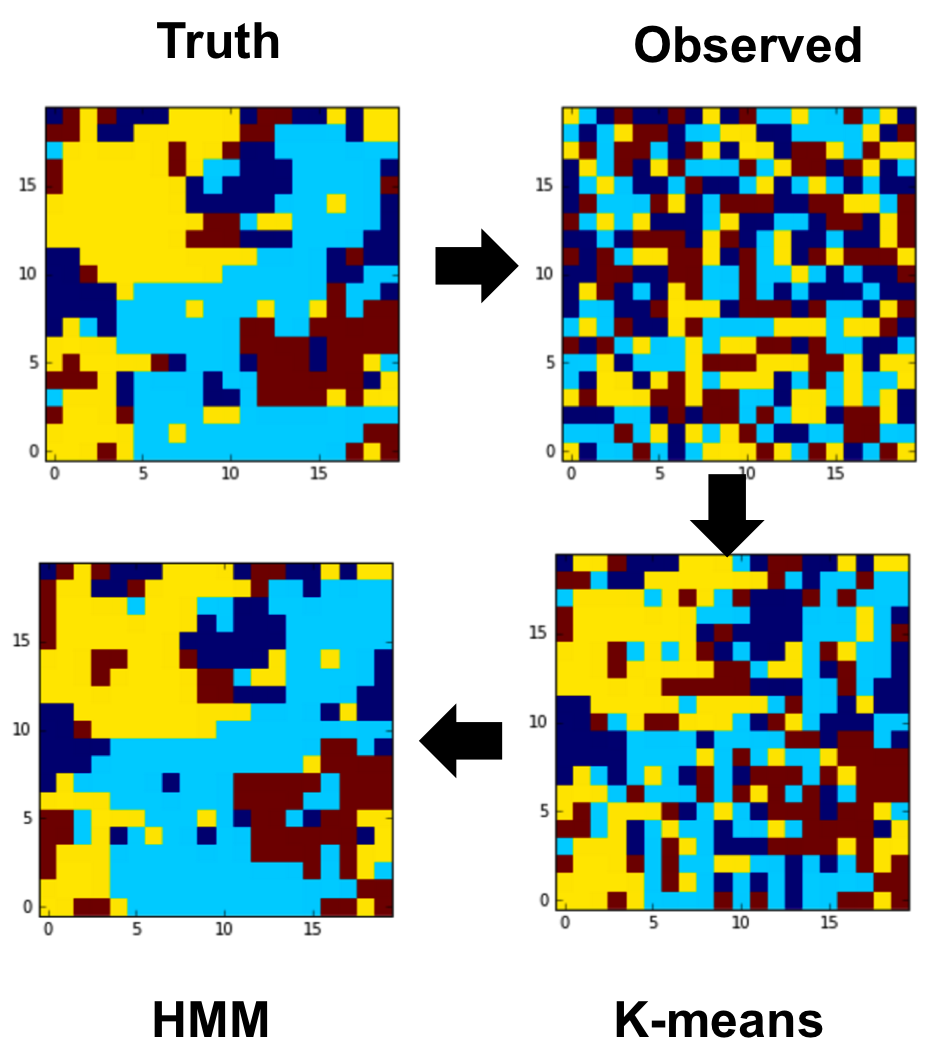
\includegraphics[width=\columnwidth]{Simulation}}
\caption{An example simulation}
\label{Simulation}
\end{center}
\vskip -0.2in
\end{figure} 


\subsection{Data generation: Observed Time Series X}

For each of the 4 networks, I generated a mean time series $u_i$ (i.e cluster means), and then created a time series $ x_i $ for each node by adding gaussian noise to its network mean time series. I tried different noise levels, and settled on one which made K-means clustering difficult. In order to visualize the time series, I used t=3 time points. (See Figure~\ref{Data}). I also experimented with using an AR model to create auto-correlated time-series, which is more representative of real fMRI data. 

\subsection{Estimation: K-Means}

After scrambling the 'true' network labels, I used a K-means algorithm (implemented by sklearn) to infer network labels (clusters). It was mildly successful, but still had assigned many pixels to the wrong network. 

\subsection{Estimation: Hidden Markov Model}

Then, I gave the K-means labels to the HMM as a starting point. Liu 2011 does this to help the HMM converge. Then the Monte-Carlo EM was performed. Most of the true network labels, as well as the underlying mean time series $\mu_i$ and $\beta$ were effectively recovered, demonstrating a correct implementation of the algorithm. 




\begin{figure}[ht]
\vskip 0.2in
\begin{center}
\centerline{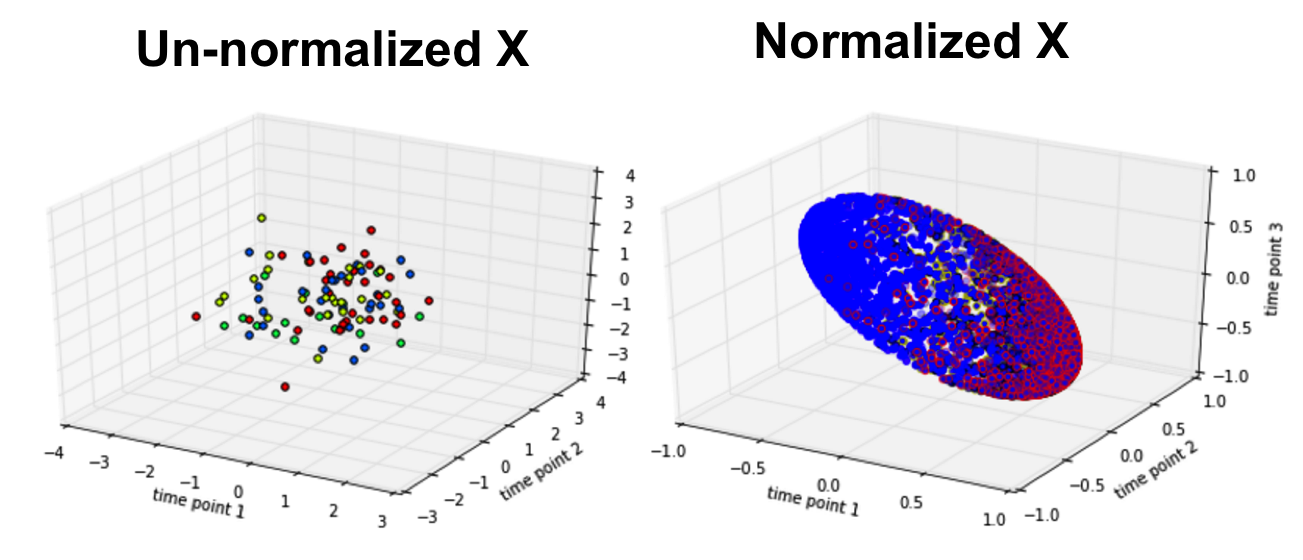
\includegraphics[width=\columnwidth]{Data}}
\caption{Examples of data used in the simulations. On the right is the data used for the previous figure. On the left, is an example of normalized data, using many more nodes to highlight the spherical nature of the data}
\label{Data}
\end{center}
\vskip -0.2in
\end{figure} 


\section{Real Data}

I applied my implementation of the Liu 2011 algorithm to an fMRI dataset I have for my research. This was done primarily to exercise what I had learned in class, but is something I may incorporate into my research in the future. Example results are found in Appendix II. 

The data are a set of 3D images collected every 2 seconds while a participant performs a task inside an MRI scanner. The images cover the whole brain and the values indicate the amount of blood flow (and thus neural activity, indirectly) at each point in time. The participants performed a 30-minute decision making task, thus there were ~1000 images collected for each subject with ~250,000 voxels (3-D pixels) for each image. My goal was to estimate functional networks for each subject during the decision making task (e.g. assign network labels to each voxel based on the time-series). 

Prior to estimating the networks, the images were masked so that only voxels around the brain were included. This limited the image size to ~60,000 voxels. Then the data was demeaned and normalized (as only relative signal matters). Finally, in a graphical data structure, voxels and their time series were assigned to nodes, and edges were created between nodes with spatially adjacent voxels. 

Like in the simulations, K-means was first applied to the data so that the HMM would be quicker to converge. I pre-specified 7 networks, because this was one stable point (along with 17 networks) in a iterative clustering procedure applied by (Yeo 2011) to hundreds of data sets. 

Finally, I ran the Monte-Carlo EM with the HMM on the dataset. With 60,000 nodes as 1000 time points, the algorithm took a very long time to run (~several hours on single core). I made a few adjustments to my original code (e.g. pre-calculating quantities that could be shared across among functions), however this did not speed up the algorithm substantially. 

The current results are that the HMM seems merely to smooth the clusters already identified by the k-means. See Figure~\ref{DatafMRI} for an example subject. Moreover, the networks are not those I expect from a neuroscience point of view. I am currently trying to improve the implementation of this algorithm on my dataset. 


\begin{figure}[ht]
\vskip 0.2in
\begin{center}
\centerline{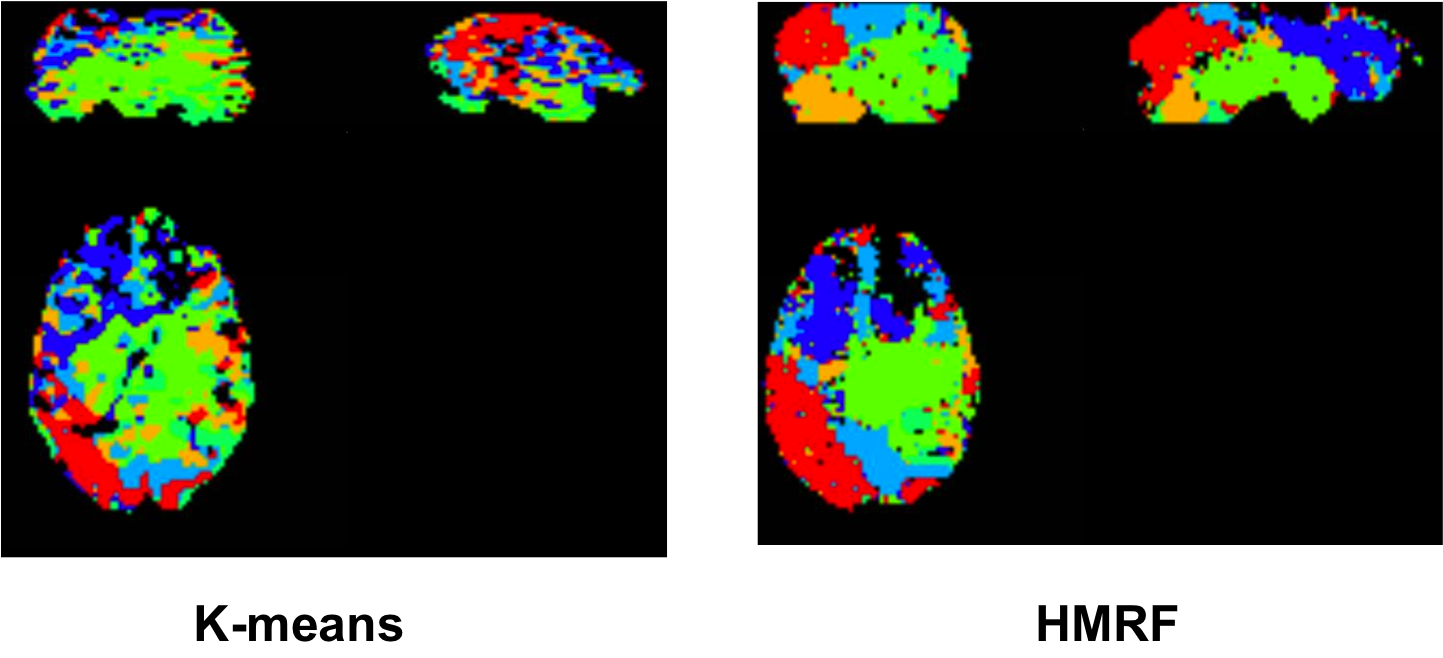
\includegraphics[width=\columnwidth]{DatafMRI}}
\caption{Examples of HMM applied to my fMRI dataset. 3 slices of the 3D image are shown}
\label{DatafMRI}
\end{center}
\vskip -0.2in
\end{figure} 



\section{Extensions}

Liu 2014 extended the Liu 2011 model by creating a hierarchical model. They proposed to connect HMM models for each participant via a group or prototype HMM network. In this hierarchical arrangement, individual participant estimation benefits from combining data across participants but only in so much as they exhibit similar networks. I started to implement this model as well (see Appendix III), although did not get a fully working simulation yet. 

Originally, I had proposed to extend the Liu 2014 model to multiple groups of subjects, however did not time to implement this extension. My research seeks to identify differences in brain function between sub-populations. Specifically, I look for differences in prefrontal/sub-cortical functioning between high and low anxious individuals (as these differences are thought to confer vulnerability to many psychiatric disorders). In this context, I could create two potential 'group' HMM networks, one for high and one for low anxious individuals. The networks can then be estimated with an additional parameter that specifies a subject's anxiety level. This parameter will determine how much a subject will contribute to the estimation high-anxious vs low anxious group map. If there are functional network differences between these sub-populations, I hope this would be a more statistically powerful method to identify them. 

Lastly, the current model of Liu 2014 is limited because it requires a pre-specified number of networks. One way to extend this limitation is to use a Dirichlet process prior to allow for the number of clusters to be inferred (with less clusters being more likely). 

\section{References} 


\begin{enumerate}
\item Wei Liu, Suyash P. Awate, Jeffrey S. Anderson, Deborah Yurgelun-Todd, P. Thomas Fletcher.  Monte Carlo Expectation Maximization with Hidden Markov Models to Detect Functional Networks in Resting-State fMRI. 2011. Machine Learning in Medical Imaging Volume 7009 of the series Lecture Notes in Computer Science pp 59-66
  \item Wei Liu, Suyash P. Awate, Jeffrey S. Anderson, and P. Thomas Fletcher. A Functional Networks Estimation Method of Resting-State fMRI Using a Hierarchical Markov Random Field. Neuroimage. 2014 October 15; 100: 520?534. doi:10.1016/j.neuroimage.2014.06.001.
  \item Yeo B, Krienen F, Sepulcre J, Sabuncu M, Lashkari D, Hollinshead M, Roffman J, Smoller J, Z�llei L,
Polimeni J, et al. The organization of the human cerebral cortex estimated by intrinsic functional
connectivity. Journal of Neurophysiology. 2011; 106:1125?1165. [PubMed: 21653723] 
\item Xiang Zhou and Scott C. Schmidler. Bayesian Parameter Estimation in Ising and Potts Models: A Comparative Study with Applications to Protein Modeling. Department of Statistical Science, Duke University
\end{enumerate}







\end{document} 


